\documentclass[xcolor=dvipsname]
{beamer}
\usepackage[utf8]{inputenc}
\usepackage{tikz}
\usetikzlibrary{arrows,shapes}
\usetikzlibrary{fadings}
\usetheme{Antibes}
\usecolortheme{beaver}
\usepackage{textpos}
\usepackage{graphicx}
\usepackage{mathtools}
\usepackage{amsmath}
\usepackage{arydshln}   %%% package for dotted line

\usepackage{algorithmic}
\usepackage{hyperref}

\mode<presentation>{}
%% preamble
\title{ Partitioning matrix and modifying min sum algorithm} 
\author[Anurag Gupta]
{\textbf {Anurag Gupta\\ Microelectronics (2015-17) \\
\footnotesize  Instructor: Prof Madhav P. Desai}}
\institute[IIT-Bombay] % (optional)
{
  IIT-Bombay\\
  Department of Electrical Engineering \\ 
  
\includegraphics[height=2cm,width=2cm]{iitb_logo}
}
\newcommand\Fontbig{\fontsize{25}{7.2}\selectfont}
%\logo{
\includegraphics[height=1.5cm]{iitb_logo.jpg}}

%\usecolortheme{dolphin}

\addtobeamertemplate{navigation symbols}{}{%
    \usebeamerfont{footline}%
    \usebeamercolor[fg]{footline}%
    \hspace{1em}%
    \insertframenumber/\inserttotalframenumber
}
\setbeamercolor{footline}{fg=blue}



\setbeamertemplate{frametitle}[default][center]



\begin{document}

%% title frame
\begin{frame}[t]
\titlepage
\end{frame}

\addtobeamertemplate{frametitle}{}{%
\begin{textblock*}{100mm}(.85\textwidth,-1cm)

\includegraphics[height=1.5cm,width=1.5cm]{iitb_logo}
\end{textblock*}}

%%%%%%%%%%%%%%%%%%%%%%%%%%%%%%%%%%%%%%%%%%%%%%%%%%%%%%%%%%%%%%%%%%%%%%%
\begin{frame}[t]
\frametitle{ Min sum decoding algorithm }                                 % and a label for
\alert{ main.c }
\begin{algorithmic}                   
    \STATE readMatrix() // reads the parity check matrix
    \STATE readCodeBlock() // reads the input code block
    \STATE \textbf{minSumDecode()}  // decode the code block 
    \STATE findAccuracy()  // check accuracy of decoded block

\end{algorithmic}
\end{frame}


\begin{frame}[t]
\frametitle{  }                                 % and a label for
\alert{ minSumDecode()	: }
\begin{algorithmic}                   
    \STATE $initialize\_aPriori() $
    \STATE $initializeMessage() $
    \WHILE{$nitr \geq Max\_nitr$}    
    	\STATE$ initialize\_aPosteriori() \Leftarrow aPriori $
   		\STATE $initializeExtrinsicInfo() \Leftarrow 0 $
  		\STATE$\textbf{checkNodeComputeEngine()}$
    	\STATE $is\_decoded = checkIsDecode()$
    	\IF{$is\_decoded = 1$}
        	\STATE break 
    	\ELSE
        	\STATE $updateMessage()$
     	\ENDIF 
     $nitr++$       	
    \ENDWHILE 
\end{algorithmic}
\end{frame}

\begin{frame}[t]
\frametitle{  }  
\begin{figure}
       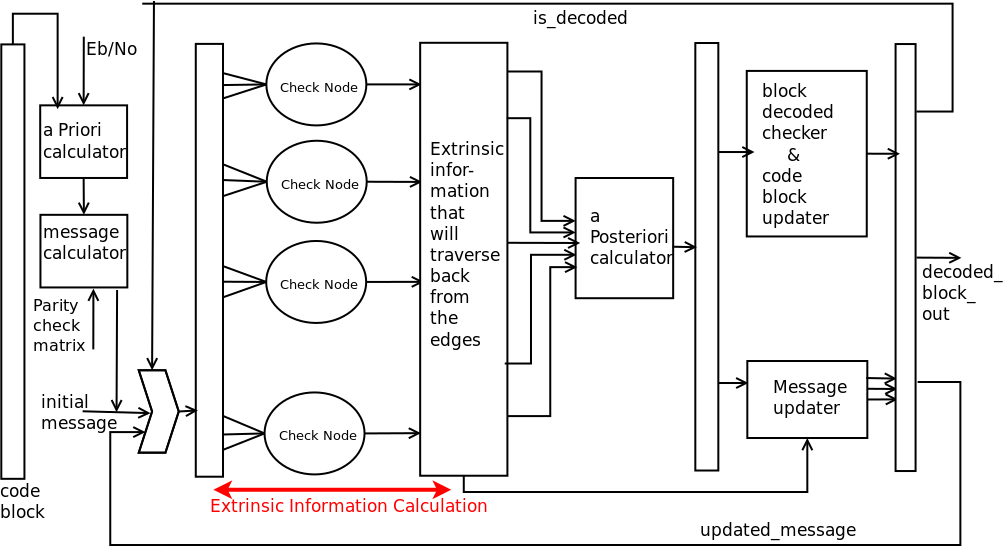
\includegraphics[height=7cm,width=11cm]{minSum}
       \end{figure}
\end{frame}

\begin{frame}[t]
\frametitle{ Algorithmic complexity at each stage }  
\begin{itemize}
\item A priori calculation	:	O(m) 
\item Message calculation 	:	O(m x p)
\item Extrinsic information calculation	: O(m x p x (p-1) ) $\approx $O($mp^{2}$)
\item A posteriori calculation : O(m x p)
\item Message updation : O(m x p)
\item block decoded calculation \& code block updation	: O(m)
\end{itemize}
\end{frame}

\section{ Modified min sum algorithm}
\begin{frame}[t]
\frametitle{ Partitioning matrix  }  
\begin{itemize}
\item After partitioning the matrix we get four matrices as follows 	:
\[
H = \left[ \begin{array}{c|c}  
H11  & H12     \\ \hline
H21  & H22     \end{array} \right] 
\] 
\item example :
\[
\begingroup % keep the change local
\setlength\arraycolsep{1pt}
\left[ \begin{array} {c|cccccccc} 
  &    c1 &   c2 &   c3 &  c4  &  c5  &  c6  &  c7  &  c8 \\ \hline
r1 &    1  &   1  &   1  &   0  &   0  &   0  &   0  &   0 \\
r2 &    0  &   0  &   0  &   1  &   1  &   1  &   0  &   0 \\ 
r3 &    1  &   0  &   0  &   1  &   0  &   0  &   1  &   0 \\
r4 &    0  &   1  &   0  &   0  &   1  &   0  &   0  &   1 \end{array} \right] 
     \Rightarrow
\left[ \begin{array} {c|cccc|cccc} 
  &    c4 &   c6 &   c7 &  c1  &  c2  &  c3  &  c8  &  c5 \\ \hline  
r2 &     1  &   1  &   0  &   0  &   0  &   0  &   0  &   1 \\
r3 &     1  &   0  &   1  &   1  &   0  &   0  &   0  &   0 \\ \hline
r1 &     0  &   0  &   0  &   1  &   1  &   1  &   0  &   0 \\
r4 &     0  &   0  &   0  &   0  &   1  &   0  &   1  &   1 \end{array} \right] 
\endgroup
\]
\item H12 and H21 are highly sparse.
\end{itemize}
\end{frame}



\begin{frame}[t]
\frametitle{ Modified min sum algorithm }                                 % and a label for
\alert{ main.c }
\begin{algorithmic}                   
    \REQUIRE Parity check matrix in row compressed form.
    \STATE readMatrixH11()
    \STATE readMatrixH12()
    \STATE readMatrixH21()
    \STATE readMatrixH22()
    \STATE readCodeBlock1()
    \STATE readCodeBlock2()
    \STATE \textbf{modifiedMinSumDecode()}
    \STATE findAccuracy()

\end{algorithmic}
\end{frame}


\begin{frame}[t]
\frametitle{  }                                 % and a label for
\alert{ modifiedMinSumDecode()	: }
\begin{algorithmic}                   
    \STATE $initialize\_aPriori(aPriori1) $
    \STATE $initialize\_aPriori(aPriori2) $
    \STATE $initializeMessage(message11) $
    \STATE $initializeMessage(message12) $
    \STATE $initializeMessage(message21) $
    \STATE $initializeMessage(message22) $
    \WHILE{$nitr \geq Max\_nitr$}    
    	\STATE$ initialize\_aPosteriori(aPosteriori1) \Leftarrow aPriori1 $
    	\STATE$ initialize\_aPosteriori(aPosteriori2) \Leftarrow aPriori2 $
   		\STATE $initializeExtrinsicInfo(ext\_info11) \Leftarrow 0 $
   		\STATE $initializeExtrinsicInfo(ext\_info12) \Leftarrow 0 $
   		\STATE $initializeExtrinsicInfo(ext\_info21) \Leftarrow 0 $
   		\STATE $initializeExtrinsicInfo(ext\_info22) \Leftarrow 0 $
   		\STATE ... 		
   		 \ENDWHILE 
\end{algorithmic}
\end{frame}

\begin{frame}[t]
\frametitle{  }                                 % and a label for
\alert{ modifiedMinSumDecode()	: }
\begin{algorithmic}   
\WHILE{...} 
\STATE ...               
\STATE$computeEngine(H11,message11,ext\_info11,trans\_info11\_12)$
\STATE$computeEngine(H22,message22,ext\_info22,trans\_info22\_12)$
\STATE$computeEngine(H12,message12,ext\_info12,trans\_info12\_11)$
\STATE$computeEngine(H21,message21,ext\_info21,trans\_info21\_22)$
\STATE$transverseCorrection(H11,transverse\_info12\_11,ext\_info11)$
\STATE$transverseCorrection(H22,transverse\_info21\_22,ext\_info22)$
\STATE$transverseCorrection(H21,transverse\_info22\_21,ext\_info21)$
\STATE$transverseCorrection(H12,transverse\_info11\_12,ext\_info12)$
\STATE$update\_aPosteriori (H11 , ext\_info11 ,aPosteriori1)$
\STATE$update\_aPosteriori (H22 , ext\_info22 ,aPosteriori2)$
\STATE$update\_aPosteriori (H12 , ext\_info12 ,aPosteriori1)$
\STATE$update\_aPosteriori (H21 , ext\_info21 ,aPosteriori2)$
\STATE ...
     	
 \ENDWHILE    


  		
\end{algorithmic}
\end{frame}


\begin{frame}[t]
\frametitle{  }                                 % and a label for
\alert{ modifiedMinSumDecode()	: }
\begin{algorithmic}   
\WHILE{...} 
\STATE ...  
\STATE$is\_decoded1 = checkIsdecoded( code\_block1 , aPosteriori1 ) $
\STATE$is\_decoded2 = checkIsdecoded( code\_block2 , aPosteriori2 ) $              
		\IF{$(is\_decoded1 \&\& is\_decoded2)== 1$}
        	\STATE break 
    	\ELSE
        	\STATE $updateMessage(ext\_info11 ,aPosteriori1 ,message11)$
        	\STATE $updateMessage(ext\_info22 ,aPosteriori2 ,message22)$
        	\STATE $updateMessage(ext\_info12 ,aPosteriori1 ,message12)$
        	\STATE $updateMessage(ext\_info21 ,aPosteriori2 ,message21)$
     	\ENDIF 
\STATE $nitr++$  
 \ENDWHILE    


  		
\end{algorithmic}
\end{frame}

\begin{frame}[t]
\frametitle{  }  
\begin{figure}
       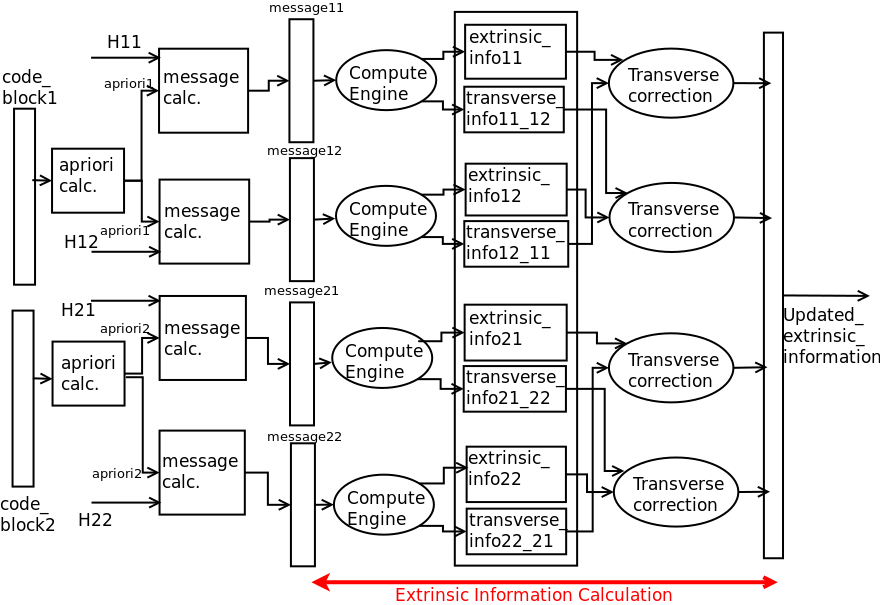
\includegraphics[height=7cm,width=11cm]{minSumModified}
       \end{figure}
\end{frame}
%-----------------------------last slide------------------------------
%---------------------------end of document---------------------------

\end{document}